\documentclass[xcolor=dvipsnames]{beamer}

\usepackage{fontspec}
\setsansfont{Bebas Neue}
\setmainfont{Nimbus Sans}

\usepackage{multicol}

\defbeamertemplate*{title page}{customized}[1][]
{
  \usebeamerfont{subtitle}
  \usebeamercolor[fg]{subtitle}

  {
    \flushright
    \setbeamercolor{author}{bg=white,fg=Black}
    \usebeamerfont{author} \rmfamily{\insertauthor\par}
    \usebeamerfont{institute}\insertsubtitle \ - \insertinstitute\par
  }

  \vspace{0.2in}

  \setbeamercolor{postit}{fg=black,bg=white}
  \begin{beamercolorbox}[sep=1em,wd=1.062\textwidth,ht=3cm,dp=3cm,center]{postit}
    \usebeamerfont{title} {\Huge \inserttitle}\par
  \end{beamercolorbox}
}

\usecolortheme[named=Black]{structure}

\setbeamertemplate{footline}[page number]{}
\beamertemplatenavigationsymbolsempty

\title{Tecnologias}

\author{Dmitry Rocha}
\subtitle{dev}

\institute{scoola}

\begin{document}

  \begin{frame}
    \titlepage
  \end{frame}

  \begin{frame}{>}
    \begin{center}
      \Huge Primeiro passo:
    \end{center}
  \end{frame}

  \begin{frame}{>}
    \begin{center}
      \Huge Onde o software irá rodar?
    \end{center}
  \end{frame}

  \begin{frame}
    \begin{center}
      \Huge Web, Desktop ou Mobile?
      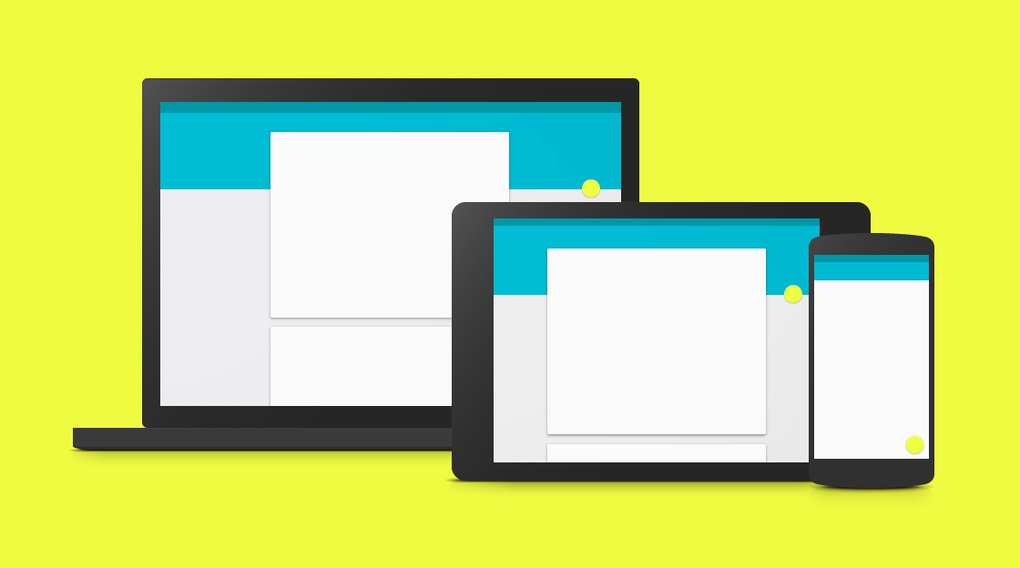
\includegraphics[width=14.5cm, height=8cm ]{images/material}
    \end{center}
  \end{frame}

  \begin{frame}
    \Huge Web.

    \normalsize Início.

    \let\thefootnote\relax\footnote{Checkpoint}
  \end{frame}

  \begin{frame}
    \Huge HTML.

    \normalsize Linguagem de marcação.
  \end{frame}

  \begin{frame}{Exemplo}
    \huge

    \begin{enumerate}
      \item HTML;
      \item "linguagem";
      \item marcação;
    \end{enumerate}
  \end{frame}

  \begin{frame}{Exemplo}
    \huge

    \begin{enumerate}
      \item \textbf{HTML};
      \item \underline{linguagem};
      \item marcação;
    \end{enumerate}
  \end{frame}

  \begin{frame}
    \normalsize Ah, então você usa\ldots

    \Huge Word?
  \end{frame}

  \begin{frame}{Exemplo}
    \vspace{1cm}

    \Huge Linguagem de \textbf{marcação}.

    \vspace{2cm}

    \normalsize

    \textbf{<p>}

    Linguagem de \textbf{<strong>}marcação\textbf{</strong>}.

    \textbf{</p>}
  \end{frame}

  \begin{frame}
    \Huge Servidor.

    \normalsize Recebe dados, processa informação e retorna ao
    usuário.

    \let\thefootnote\relax\footnote{Checkpoint}
  \end{frame}

  \begin{frame}{Exemplo}
    \Huge Formulário.

    \normalsize Nome+Idade, retorna o ano de nascimento.
  \end{frame}

  \begin{frame}{Parte fácil?}
    \begin{center}
      \Large Na teoria a parte fácil foi fazer

      \vspace{1cm}

      \Huge as questões "tradicionais"

      \vspace{1cm}

      \Large Usando formulários, links, \ldots
    \end{center}
  \end{frame}

  \begin{frame}{Parte fácil?}
    %\begin{center}
      \Huge Tipos de questões:

      \begin{enumerate}
        \item Multipla escolha;
        \item subjetiva;
        \item completar;
      \end{enumerate}

      \let\thefootnote\relax\footnote{Checkpoint}
    %\end{center}
  \end{frame}

  \begin{frame}{Parte fácil?}
    \begin{center}
      \Large Parte fácil?

      \Huge Problema?

      \Large Será?
    \end{center}
  \end{frame}

  \begin{frame}{Exemplo}
    \begin{center}
      \large Questões de múltipla escolha ou completar.
    \end{center}

    \pause

    \huge O professor sempre cria a primeira alternativa como resposta certa\ldots

    \pause

    \begin{center}
      \Huge \ldots com o tempo percebe-se que sempre a primera alternativa é
      a resposta certa.
    \end{center}
  \end{frame}

  \begin{frame}{Problema?}
    \begin{center}
      \huge As questões de {\Huge multipla escolha} e {\Huge completar}

      tem que ter as resposta em

      \textbf{ordem aleatória}.
    \end{center}
  \end{frame}

  \begin{frame}{Problema?}
    %\begin{center}

      \Huge Subjetiva:

      \vspace{1cm}

      \LARGE

      remover acentos,

      espaços extras e

      maiúscula/minúscula

      \let\thefootnote\relax\footnote{Checkpoint}
    %\end{center}
  \end{frame}

  \begin{frame}
    \begin{center}
      \Huge Problema? Mesmo?
    \end{center}
  \end{frame}

  \begin{frame}
    \begin{center}
      \Large Arrastar e soltar.

      \vspace{1cm}

      \LARGE {\rmfamily \%} Canvas {\rmfamily \&\&} javascript

      \vspace{1cm}

      \Large Traçado, velocidade, pressão.
    \end{center}
  \end{frame}

  \begin{frame}
    \begin{center}
      \Large Testes.

      \vspace{1cm}

      \LARGE Padrão de projeto.

      \vspace{1cm}

      \Large Cópia de segurança das informações.
    \end{center}
  \end{frame}

  \begin{frame}
    \begin{center}
      
\includegraphics[width=\textwidth, height=\textheight]{images/013-stefan-asafti-marcas-cartoon-isso-e-tudo}
    \end{center}
  \end{frame}
\end{document}
